% !TEX root = ../thesis_main.tex
\chapter{Coherent Processes of Single-Wall Carbon Nanotubes}

\section{Introduction}


{\color{red} UNFINISHED}Talking about ultrafast optical switching. SWCNTs quite suited to this due to fast carrier dynamics, unlike those of inorganic semicondutors \cite{maeda2006gigantic}. Useful for optical switching processes such as those induced by the optical Stark effect. For pump detuned below $E_{11}$ energy transition, the $E_{11}$ peak experiences a blue-shift that occurs only during the presence of the optical pump. For sufficiently large detunings, this blue-shift $\Delta E_{11}$ can be expressed as
%
\begin{equation}
		\Delta E_{11} = \sqrt{(\hbar \Omega_R)^2 + \Delta^2} - \Delta,
\end{equation}
%
which includes {\color{red} UNFINISHED}. However, multi-photon processes occur that lead to the creation of real carriers which can photo-bleach the $E_{11}$ resonance if enough carriers are created and thereby limit the performance of the optical switching.

We can quantify the performance of optical switching by using the term reversibility to describe the effect on which non-coherent processes on the optical switching. Here, reversibility is defined as
%
\begin{equation}
 	\text{Rev} = \dfrac{\Delta T_\text{peak} - \Delta T_\text{base}}{\Delta T_\text{peak}},
\end{equation}
%
which includes the baseline transmission $\Delta T_\text{base}$ that represents the average of the transmission before and after switching occurs whereas, the peak change in transmission $\Delta T_\text{peak}$ only measures the coherent changes in transmission due to the optical Stark effect. Furthermore, $\Delta T_\text{base}$ accounts for changes in trasmission due to the creation of real carriers. It also implicitly depends on other parameters such as the detuning and fluence of the optical pump as well as the time delay between incident pump pulses.

{\color{red} UNFINISHED} Theory developed by Professor Mackillo Kira and his student Weiwei Jiang. Here, they solve Maxwell-semiconductor Bloch equations \cite{kira2011semiconductor} in a self-consistent manner for (6,5) SWCNTs. These calculations also account for non-coherent processes to help describe the dephasing kinetics which may affect the reversibility of the optical switching dynamics. In a typical scenario, the optical pump pulse creates an electron-hole distribution $f_\text{k}^\text{e(h)}$, via multi-photon processes, as well as a coherent polarization $P_\text{k}$ at the carrier momentum $\hbar k$.

Shortly after, $P_\text{k}$ begins to dephase due to scattering events within the $f_\text{k}^\text{e(h)}$ distribution as a result of Coulomb interactions. From a phenomenological perspective, this dephasing can be described by an instantenous decay
\begin{equation}
	\dfrac{\partial}{\partial t} P_\text{k}(t) \Big|_\text{instant} = -\gamma P_\text{k}(t),
\end{equation}
which is parametrized by a dephasing constant $\gamma$ that implicitly accounts for quantum-kinetic scattering. However, after taking a full account of the quantum phenomena underlying these behaviors
\begin{equation}
	\dfrac{\partial}{\partial t} P_\text{k}(t) \Big|_\text{Q. Memory} = -\gamma \int^{t}_{\infty} dt' \left[ \exp\left\{ - \frac{\small i}{ \small \hbar} \hat{\mathcal{H}}_\text{ex}(t-t') \right\} P(t') \right]_\text{k} \exp \left(- \frac{t-t'}{T_\text{QM}} \right)
\end{equation}

\begin{equation}
	\left[ \hat{\mathcal{H}}_\text{ex} \right]_\text{k, K}= \delta_\text{k, K} \tilde{E_\text{k}} - (1 - f_\text{k}^\text{e} - f_\text{k}^\text{h}) V_\text{k-K}
\end{equation}


\section{Experimental Results}

\begin{figure}[H]
	\centering
	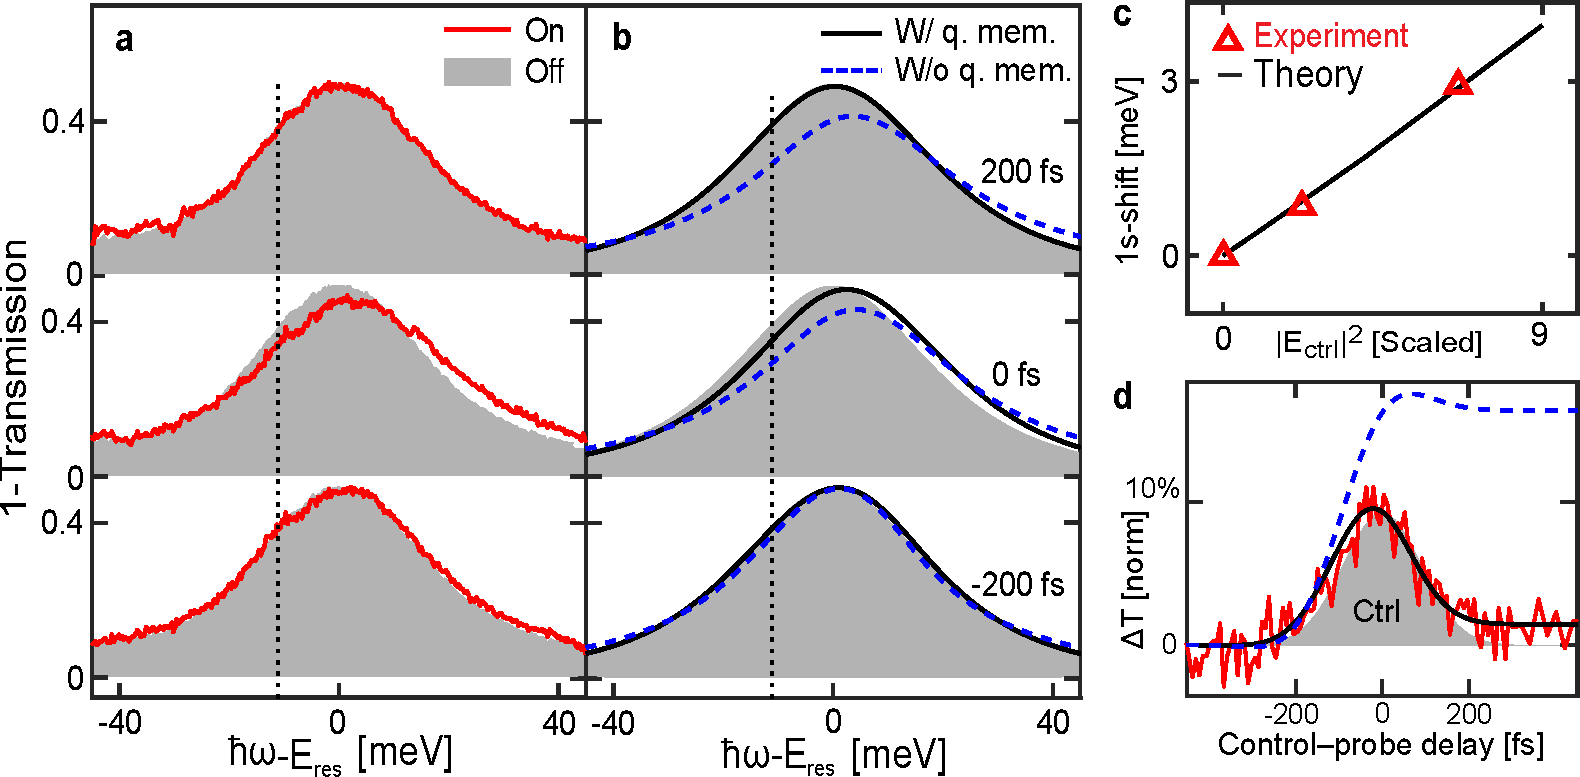
\includegraphics[height=2.4in]{images/chapter_coherent/nonresonant}
	\caption{{\color{red}UNFINISHED} Reproduced from Ref.\ \cite{mack2019}}
\end{figure}

\begin{figure}[ht]
	\centering
	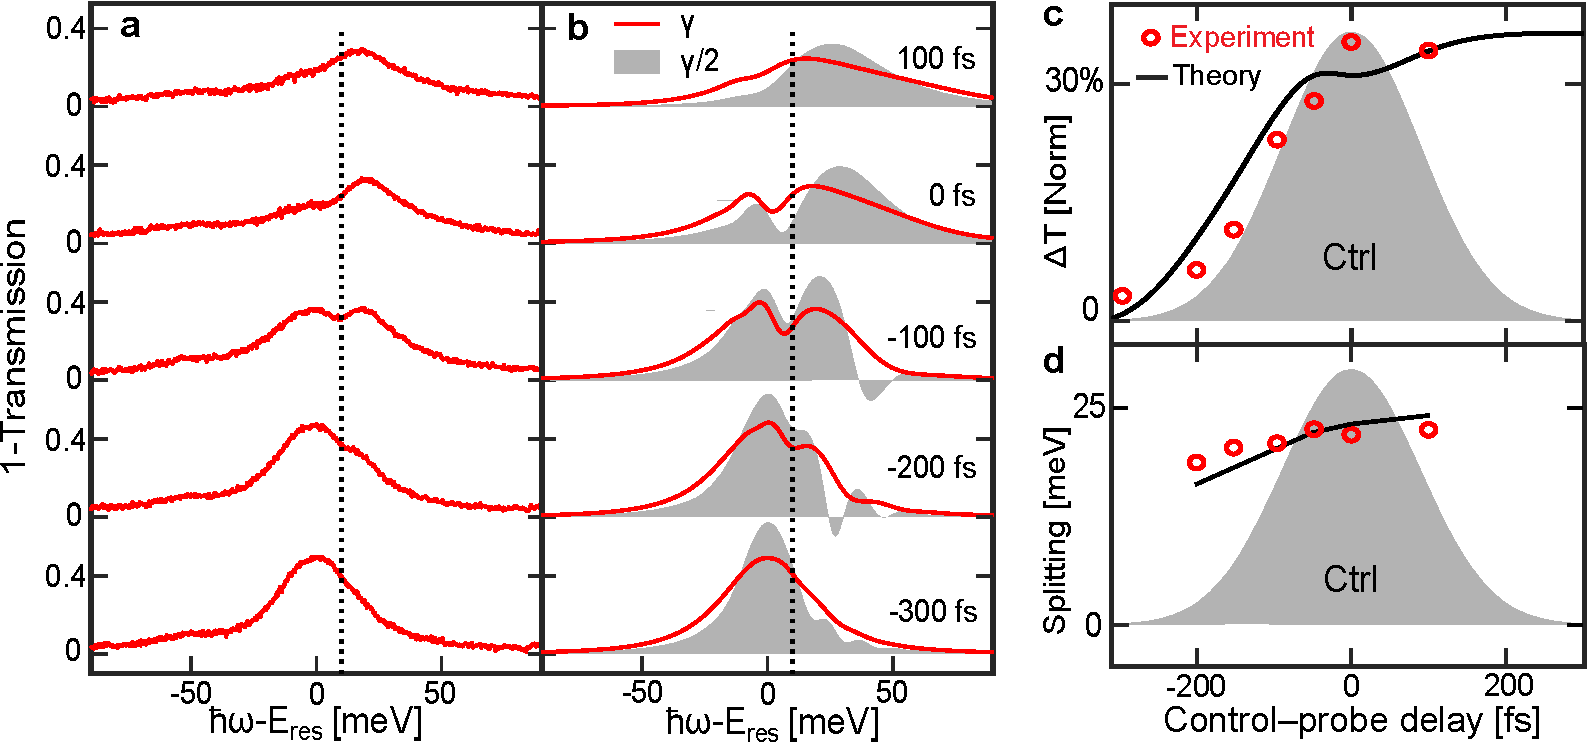
\includegraphics[height=2.4in]{images/chapter_coherent/resonant}
	\caption{{\color{red}UNFINISHED} Reproduced from Ref.\ \cite{mack2019}}
\end{figure}

\clearpage

\begin{figure}[ht]
	\centering
	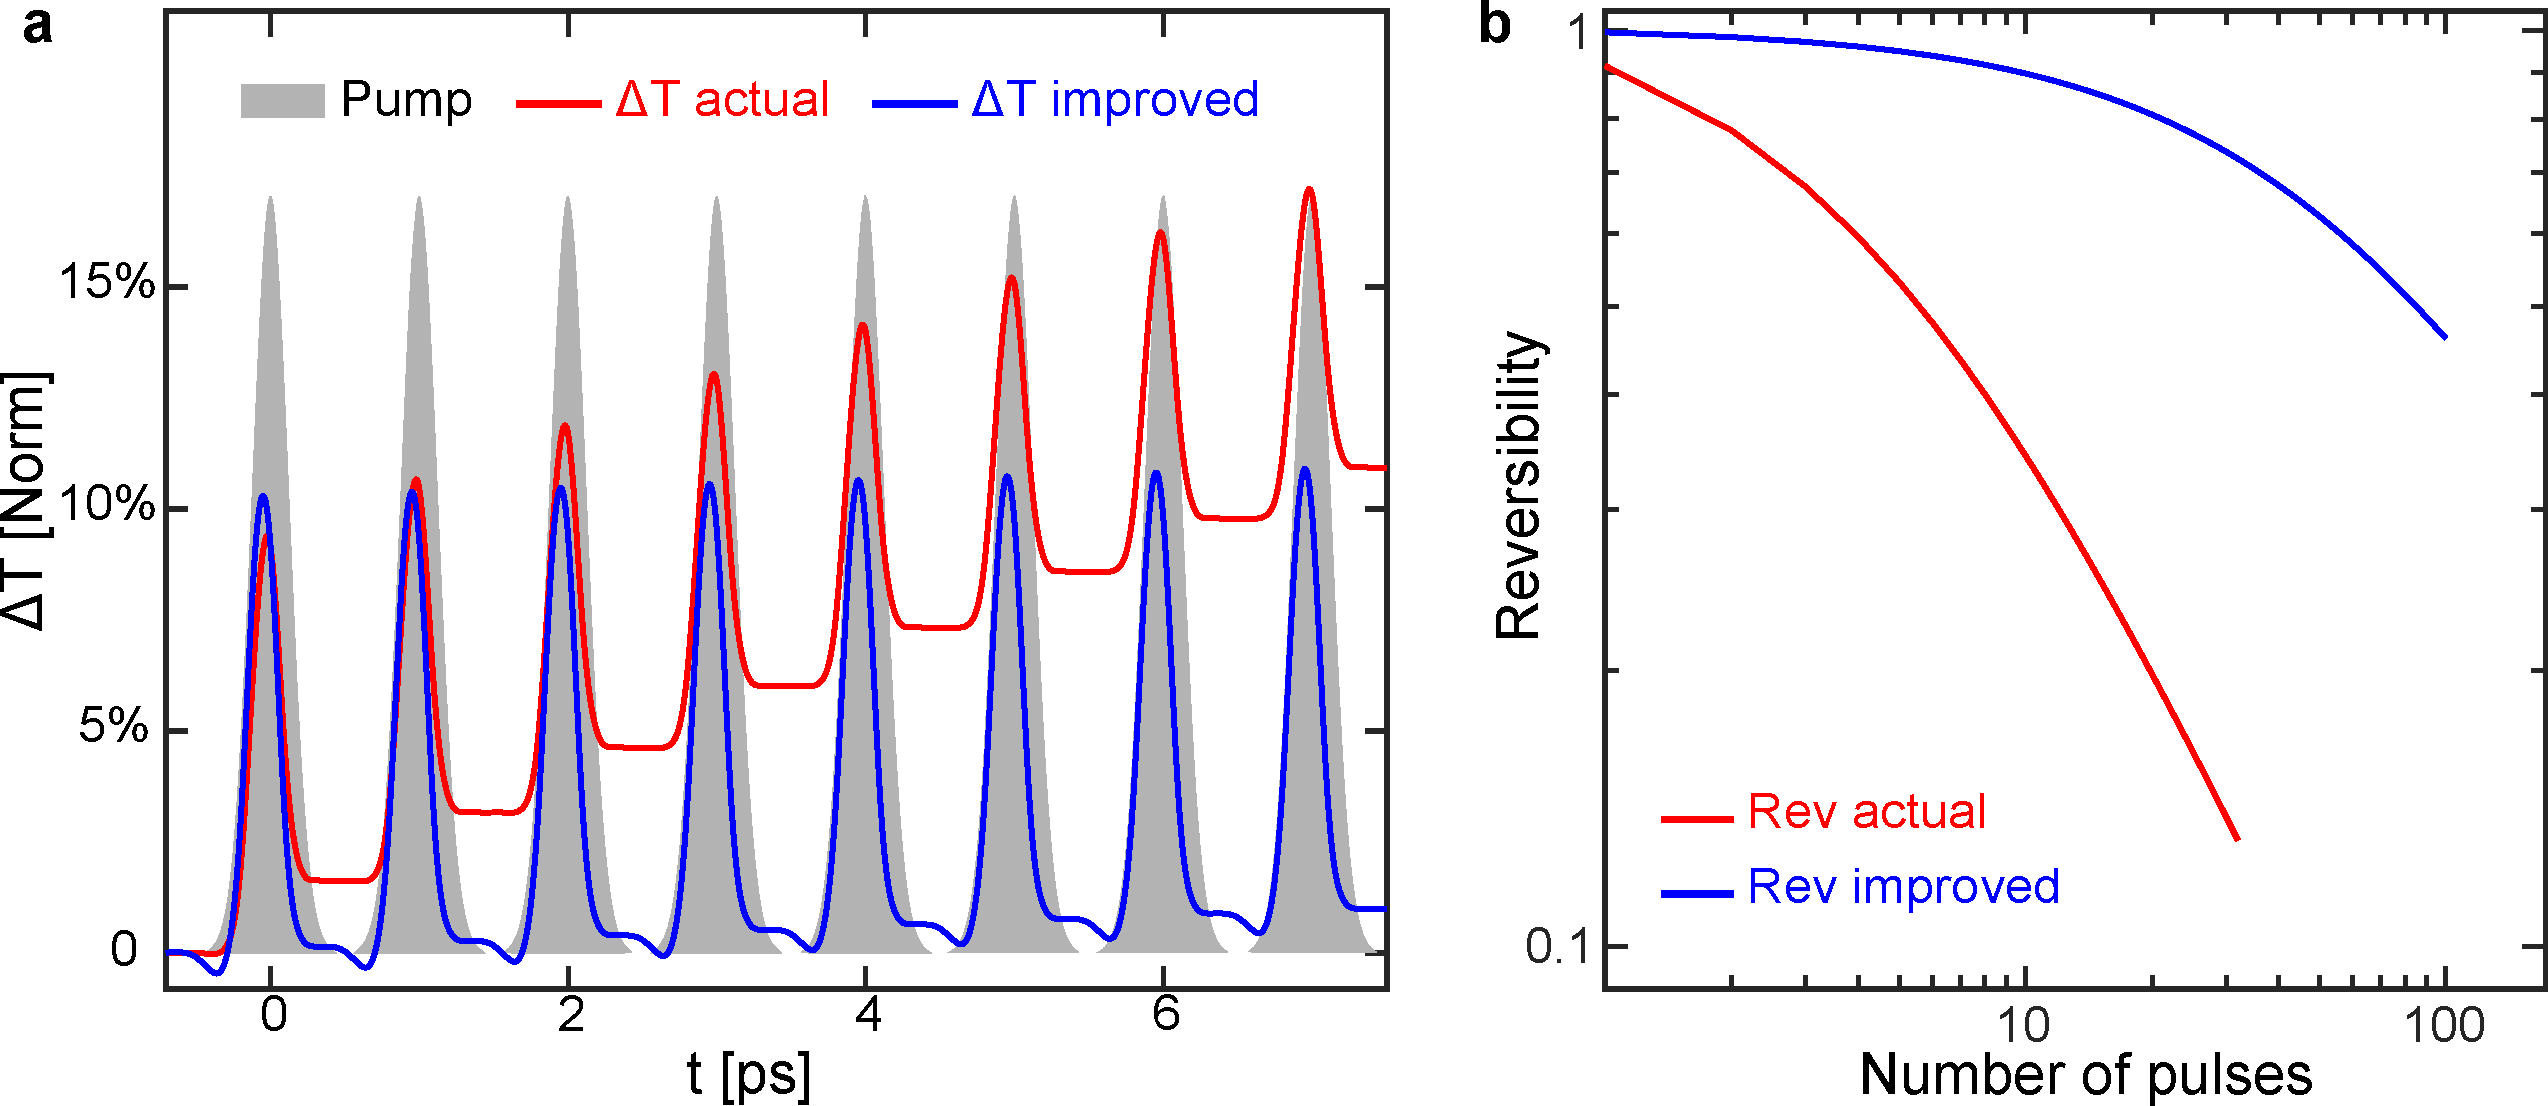
\includegraphics[height=2.4in]{images/chapter_coherent/switching_reversibility}
	\caption{{\color{red}UNFINISHED} Reproduced from Ref.\ \cite{mack2019}}
\end{figure}




\section{Discussion}

\section{Conclusions}
